\DiaryEntry{Groups - Cosets}{2016-03-25}{Algebra}

Consider a groupg G with a subgrop H; A left coset of H with
representative \(a \in G\) is defined as

\[
aH = \{a \star h: h \in H \}
\]

That is, we choose \textbf{any} element a from G and create the set by
performing the group operation \(\star\) on a and every element from H.

Since the group operation is not commutative in general, we can
analoguously define a right coset according to

\[
Ha = \{h \star a : h \in H \}
\]

Note that cosets are sets and \textbf{not} groups.

\subsection{Example $\mathbb{Z}_6$}\label{example-mathbbz_6}

Consider the group \(G = \mathbb{Z}_6\) with element \(0,1,2,3,4,5\) and
modulo-6 addition as group operation. The subgroup is \(H = \{0,3\}\).

Make a quick check that H is really a subgroup: (i) It contains the
identitiy element \(0\), (ii) it is closed under addition modulo-6 as
\(3 \star 3 = 0\), and (iii) every group element has an inverse:
trivially for group element \$0\$0, and the inverse of \(3\) is \(3\);
see (ii).

Since the group operation is commutative, left and right cosets are the
same; we have

\begin{align*}
0 + H &= \{0,3\} \\
1 + H &= \{1,4\} \\
2 + H &= \{2,5\} \\
3 + H &= \{3,0\} \\
4 + H &= \{4,1\} \\
5 + H &= \{5,2\}
\end{align*}


First note that several cosets are equal (as cosets are sets, they are
equal when they contain the same elements). Simplifying things we obtain


\begin{align*}
0 + H &= 3 + H = \{0,3\} \\
1 + H &= 4 + H = \{1,4\} \\
2 + H &= 5 + H = \{2,5\} \\
\end{align*}


The Figure below shows the corresponding Cayley diagram with G (black)
and H (red), and the cosets. The cosets have the original structure of
the underlying subgroup; however they are ``shifted'' to a new posiiton.
The Figure and the example above also show that cosets are not groups in
general; e.g.~the coset \(\{1,4\}\) is a set but not a group.

\begin{figure}[H]
\centering
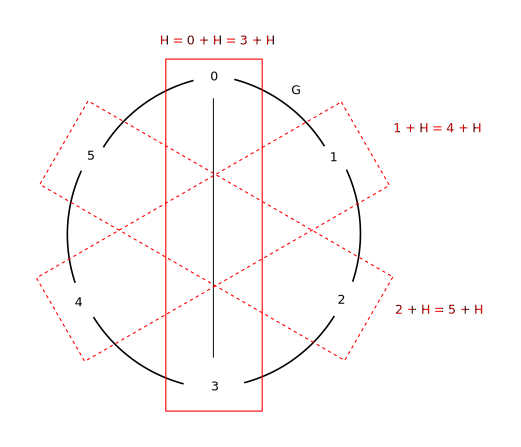
\includegraphics[scale=0.7]{images/groups_05_1.png}
\caption{Page1}
\end{figure}

Since cosets are sets, two cosets \(Ha\) and \(Hb\) are equal when
\(a \in H b\) follows from \(a \in H a\) and vice versa.

\subsection{Coset Characteristics}\label{coset-characterisitcs}

\subsubsection{Coset Membership}\label{coset-membership}

We have the following fact:

\[
a \in Hb \rightarrow Ha = Hb
\]

Let \(x \in Ha\); therefore we have \(x = h_2 a\) where \(h_2\) is some
element of H. But we also have that \(a \in Hb\) which implies that
\(a = h_1 b\) and if we combine that, we get
\(x = h_2 a = h_2 ( h_1 b) = (h_2 h_1) b\). The product \(h_2 h_1\) is
clearly an element of \(H\); therefore \(x \in Hb\). This proves that
every \(x \in Ha\) is also contained in \(Hb\); if we make the same
argument with exchanged roles, we also find that every \(x \in Hb\) is
also contained in \(Ha\).

From this follows that cosets are either disjoint or equal (contain the
same elements). There is no thing as two cosets having only some
elements in common ``ganz oder gar nicht''.

\subsubsection{Coset Partitioning}\label{coset-partitioning}

We have the following theorem: The family of all cosets \(Ha\), as a
ranges of G, is a partition of G.

In the exmaple above, the three cosets \(0 + H, 1 + H, 2 + H\) partition
the group G.

We can prove this in two steps: First we show that two cosets Ha and Hb
are either disjoint or equal. If they are disjoint then we are done. If
not, then choose \(x \in Ha \cap Hb\). From \(x \in Ha\) follows
\(x = h_1 a\) and from \(x \in Hb\) follows \(x = h_2 b\). We can equal
these two and arrive at \(h_1 a = h_2 b\) which we can solve for a as
\(a = (h_1^{-1} h_2) b\). This shows that \(a \in Hb\) (\(h_1^{-1} h_2\)
is clearly an element of H) and from the reasoning in the previous
Subsection, it follows that \(Ha = Hb\).

Second part of the proof is that \textbf{every} element of G is
contained in one of the cosets of H. Choose \(c \in G\) and we can write
this as \(c = c1\) and \(1 \in H\) (otherwise H would not be a
subgroup!). Therefore, \(c = Hc\) and we are done.

\subsubsection{Coset Size}\label{coset-size}

Next we show that all cosets (of a given subgroup H) have the same size
as the subgroup H. Stated differently, there is a one-to-one
correspondence from H to Ha.

We choose the function \(f:H \rightarrow Ha\) as \(f(h) = ah\); here a
remains fixed and h varies. This function is both injective and
surjective:

\begin{itemize}
\item
  It is injective (i.e.~it never maps distinct values \(h\) into the
  same values \(f(h)\)), because if \(f(h_1) = f(h_2)\), then
  \(ah_1 = ah_2\) and therefore \(h_1 = h_2\).
\item
  It is surjective (i.e.~no element from the image is left out), because
  every element of the image Ha can be expressed as \(ha\) (with some
  \(h \in H\)).
\end{itemize}

\subsubsection{Lagrange's Theorem}\label{lagranges-theorem}

We can combine what we have so far: We have a group G and a subgroup H.
G is partitioned by the cosets of H and all these cosets have the same
size. Therefore, the number of elements in G equals the number of
elements in H (or any coset of H) times the number of distinct cosets of
H.

Stated differently, we can say that the order of any subgroup H of a
group G divides the order of G.

If we think of the example above, \(\mathbb{Z}_6\) has 6 elements and
can therefore have subgoups of size 2 and 3.

In the special case of a group with prime order p, only subgroups of
size 1 and p exist. The latter is the group itself. Therefore, a group
with prime order has p subgroups each having order 1. Such a (sub)group
is a cyclic group; and G is then also a cyclic group. Furthermore, any
group element \(a \in G\) forms a cyclic group with equals G with \(a\)
being the generator: \(\langle a \rangle = G\) for any \(a \in G\).

\subsection{Left and Right Cosets, Normal
Subgroups}\label{left-and-right-cosets-normal-subgroups}

A left coset is defined as

\[
aH = \{a \star h: h \in H \}
\]

The interpretation is as follows: We start at the coset
``representative'' \(a\), multiply each subgroup element and the result
forms the left coset.

A right coset is defined as

\[
Ha = \{h \star a : h \in H \}
\]

and can be interpreted that we start in an element of the subgroup
\(H\), and multiply with \(a\). Doing this for all elements of \(H\)
yields the right coset.

The Figure below shows the concepts. The left coset (shown on the left
:-) ) shows the subgroup \(H\) ``surrounding'' the identity element
\(e\). Considering the left coset \(aH\) means shifting every subgroup
element of \(H\) by the element \(a\).

The right coset (shown on the right) starts with the subgroup \(H\):
Every element of the subgroup (which includes the identity element
\(e\)) is then shifted by \(a\), yielding the coset
\(Hg = \{g, h_1 a, h_2 a, h_3 a, \ldots\}\).

\begin{figure}[H]
\centering
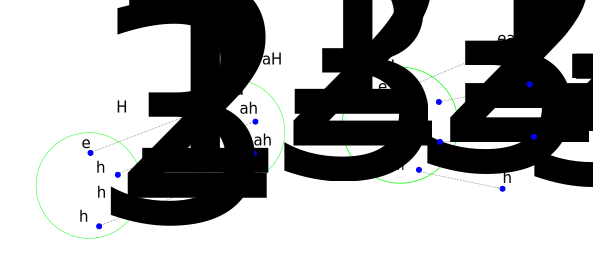
\includegraphics[scale=0.7]{images/groups_05_2.png}
\caption{Page1}
\end{figure}

\subsubsection{Example: Dihedral Group $D_3$}\label{example-dihedral-group-d_3}

In order to beat the examples to death, we consider the Dihedral Group
\(D_3\), defined by the three characteristic equations
\(r^3 = e, s^2=1, srs=r^{-1}\). We use the convention that the operation
\(a\star b\) is to be read from left to right = We start at element a
and apply b.

In the Cayley Diagram shown below, the identities at the points A and B
are interesting. In A, we have \(r^2 s = sr\): Right-multiplying with
\(s\), we obtain \(r^2 s^2 = srs \rightarrow r^2 = r^{-1}\). In B, we
have \(sr^2 = rs\); left-multiplying with \(s\) we obtain
\(s^2 r^2 = srs \rightarrow r^2 = r^{-1}\).

\begin{figure}[H]
\centering
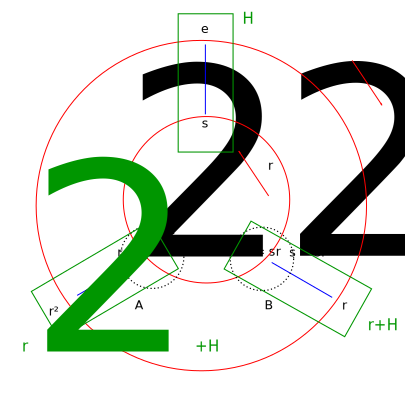
\includegraphics[scale=0.7]{images/groups_05_3.png}
\caption{Page1}
\end{figure}

Next we need a subgroup - the set \(H=\{e, s\}\) is one (as \(s^2=e\)).
The left cosets of \(H\) are

\begin{itemize}
\item
  \(rH = \{re, rs\} = \{r, rs\}\)
\item
  \(r^2H = \{r^2e, r^2s\} = \{r^2, r^2s\}\)
\item
  \(sH = \{s, s^2\} = \{e, s\} = H\)
\item
  \(rsH = \{rs, rs^2\} = rH\)
\item
  \(r^2sH = \{r^2s, r^2s^2\} = r^2H\)
\end{itemize}

The right cosets of \(H\) are

\begin{itemize}
\item
  \(Hr = \{er, sr\} = \{r, sr\}\)
\item
  \(Hr^2 = \{er^2, sr^2\} = \{r^2, sr^2\}\)
\item
  \(Hs = \{s, s^2\} = H\)
\item
  \(Hrs = \{rs, srs\} = \{rs, r^2\} = Hr^2\)
\item
  \(Hr^2s = \{r^2s, sr^2s\} = \{r^2s, r\} = Hr\)
\end{itemize}

It can be seen that the left cosets (shown in green) preserve the
structure of the subgroup, whereas the right cosets distribute elements
across the Cayley diagram.

Next we consider a different subgroup \(H' = \{e, r, r^2\}\). The left
cosets are

\begin{itemize}
\item
  \(rH' = \{r, r^2, e\} = H'\)
\item
  \(r^2H' = \{r^2, e, r\} = H'\)
\item
  \(sH' = \{s, sr, sr^2\}\)
\item
  \(rsH' = \{rs, rsr, rsr^2\} = \{rs, s, sr^2\} = sH'\)
\item
  \(r^2sH' = \{r^2s, r^2sr, r^2sr^2\} = \{r^2s, sr^2, s\} = sH'\)
\end{itemize}

The right cosets are

\begin{itemize}
\item
  \(H'r = \{r, r^2, r^3\} = rH'\)
\item
  \(H'r^2 = \{r^2, e, r\} = r^2H'\)
\item
  \(H's = \{s, rs, r^2s\} = sH'\)
\item
  \(H'rs = \{rs, r^2s, r^3s\} = rsH'\)
\item
  \(H'r^2s = \{r^2s, r^3s, r^4s\} = r^2sH'\)
\end{itemize}

Note that the left and right cosets are equal; therefore, the subgroup
H' is a normal subgroup.
